\documentclass[tikz, border=6pt]{standalone}
\IfFileExists{lmodern.sty}{\usepackage[T1]{fontenc}\usepackage{lmodern}}{}
\usepackage{amsmath,amssymb,bm}
\usepackage[scaled=0.95]{helvet}
\usetikzlibrary{arrows.meta}
\definecolor{Blue}{HTML}{3A76D8}
\definecolor{Green}{HTML}{3BA55C}
\definecolor{Purple}{HTML}{8459D1}
\definecolor{Ink}{HTML}{1F2937}
\tikzset{
  block/.style={/utils/exec={\colorlet{pytikzarg}{#1}}, draw=pytikzarg!78!black, fill=pytikzarg!14, rounded corners=3pt, align=center, inner sep=5pt, minimum height=8mm, minimum width=20mm},
  block/.default=Blue,
}
\begin{document}
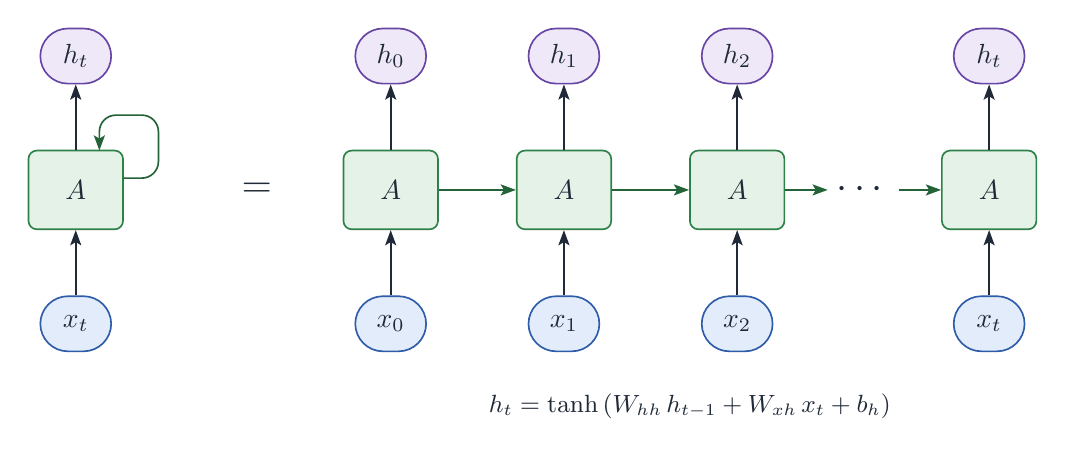
\begin{tikzpicture}[color=Ink, execute at begin picture={\sffamily}, line width=0.6pt, >={Stealth[length=5.5pt, width=4pt, inset=1.2pt]}, line join=round]
  \node[block=Green, minimum width=1.2cm, minimum height=1cm] (n1) at (0,0) {$A$};
  \node[block=Blue, minimum width=0.9cm, minimum height=0.7cm, rounded corners=10pt] (n2) at (0,-1.7) {$x_t$};
  \draw[->] (n2) -- (n1);
  \node[block=Purple, minimum width=0.9cm, minimum height=0.7cm, rounded corners=10pt] (n3) at (0,1.7) {$h_t$};
  \draw[->] (n1) -- (n3);
  \draw[->, rounded corners=6pt, color=Green!60!black] (0.6,0.15) -- (1.05,0.15) -- (1.05,0.95) --
      (0.3,0.95) -- (0.3,0.5);
  \node[font=\Large] at (2.3,0) {$=$};
  \node[block=Green, minimum width=1.2cm, minimum height=1cm] (n4) at (4,0) {$A$};
  \node[block=Blue, minimum width=0.9cm, minimum height=0.7cm, rounded corners=10pt] (n5) at (4,-1.7) {$x_0$};
  \draw[->] (n5) -- (n4);
  \node[block=Purple, minimum width=0.9cm, minimum height=0.7cm, rounded corners=10pt] (n6) at (4,1.7) {$h_0$};
  \draw[->] (n4) -- (n6);
  \node[block=Green, minimum width=1.2cm, minimum height=1cm] (n7) at (6.2,0) {$A$};
  \node[block=Blue, minimum width=0.9cm, minimum height=0.7cm, rounded corners=10pt] (n8) at (6.2,-1.7) {$x_1$};
  \draw[->] (n8) -- (n7);
  \node[block=Purple, minimum width=0.9cm, minimum height=0.7cm, rounded corners=10pt] (n9) at (6.2,1.7) {$h_1$};
  \draw[->] (n7) -- (n9);
  \node[block=Green, minimum width=1.2cm, minimum height=1cm] (n10) at (8.4,0) {$A$};
  \node[block=Blue, minimum width=0.9cm, minimum height=0.7cm, rounded corners=10pt] (n11) at (8.4,-1.7) {$x_2$};
  \draw[->] (n11) -- (n10);
  \node[block=Purple, minimum width=0.9cm, minimum height=0.7cm, rounded corners=10pt] (n12) at (8.4,1.7) {$h_2$};
  \draw[->] (n10) -- (n12);
  \node[block=Green, minimum width=1.2cm, minimum height=1cm] (n13) at (11.6,0) {$A$};
  \node[block=Blue, minimum width=0.9cm, minimum height=0.7cm, rounded corners=10pt] (n14) at (11.6,-1.7) {$x_t$};
  \draw[->] (n14) -- (n13);
  \node[block=Purple, minimum width=0.9cm, minimum height=0.7cm, rounded corners=10pt] (n15) at (11.6,1.7) {$h_t$};
  \draw[->] (n13) -- (n15);
  \draw[->, color=Green!60!black] (n4) -- (n7);
  \draw[->, color=Green!60!black] (n7) -- (n10);
  \draw[->, color=Green!60!black] (n10) -- (9.55,0);
  \node[font=\Large] at (10,0) {$\cdots$};
  \draw[->, color=Green!60!black] (10.45,0) -- (n13);
  \node[font=\small] at (7.8,-2.75) {$h_t = \tanh\left(W_{hh}\,h_{t-1} + W_{xh}\,x_t + b_h\right)$};
\end{tikzpicture}
\end{document}
